% 上机实验报告02 - 数据挖掘与机器学习
% 请将“学号姓名”替换为实际学号与姓名

\documentclass[12pt,a4paper]{article}
\usepackage[UTF8]{ctex}
\usepackage{geometry}
\usepackage{amsmath,amssymb}
\usepackage{graphicx}
\usepackage{booktabs}
\usepackage{float}
\usepackage{hyperref}
\usepackage{enumitem}
\usepackage{caption}

\geometry{left=2.5cm,right=2.5cm,top=2.5cm,bottom=2.5cm}
\setlength{\parindent}{2em}
\graphicspath{{result/}}

\title{\textbf{上机实验报告02\\数据挖掘与机器学习}}
\author{学号：\underline{1043220122} \quad 姓名：\underline{林鑫} \quad 班级：\underline{信计2302班}}
\date{}

\begin{document}
\maketitle
\thispagestyle{empty}
\vspace{1em}

% ========== 一、实验目的 ==========
\section{实验目的}
本实验旨在利用Python对数据进行探索性数据分析，通过数据清洗、可视化、统计分析及简单建模，掌握数据处理的基本方法。实验可参考Script02.ipynb中的分析思路（如变量关系分析、残差图、回归系数计算、同方差与异方差检验等），将其应用于其它数据。

% ========== 二、实验环境 ==========
\section{实验环境}
编程语言：Python

主要库：pandas 数据处理；numpy 数值计算；matplotlib \& seaborn 数据可视化；sklearn 机器学习工具（用于评估指标）；scipy 统计分析（如正态性检验）；statsmodels 异方差检验（Breusch-Pagan）等。

% ========== 三、数据描述 ==========
\section{数据描述}
\paragraph{数据来源与样本} 本实验使用沪深300指数最近三年日频数据（\texttt{沪深300\_最近三年.csv}）。数据由 \texttt{get\_data.py} 通过腾讯财经接口（\texttt{web.ifzq.gtimg.cn}）拉取沪深300日K线前复权数据并导出为 CSV 得到。原始数据为交易日级别的行情数据，经清洗后共 727 条有效记录，时间跨度为 2023-03-13 至 2026-03-13，覆盖约三年交易日，样本量足以进行描述性统计、相关性与简单回归分析。

\paragraph{原始字段说明} 原始数据包含字段：\textbf{日期}（交易日期）、\textbf{收盘}（当日收盘指数）、\textbf{开盘}（当日开盘指数）、\textbf{高}（当日最高）、\textbf{低}（当日最低）、\textbf{交易量}（字符串形式，如 ``123533.67K''）、\textbf{涨跌幅}（百分比字符串，如 ``0.24\%''）。从原始字段可知：收盘价在约 3160--4790 点之间波动，涨跌幅与交易量反映市场活跃程度与波动幅度，需经类型转换后方可参与数值计算。

\paragraph{预处理后变量} 预处理后用于分析的数值型变量包括：收盘价、开盘价、最高、最低；交易量转为 \texttt{volume\_k}（单位：千）；日收益率 \texttt{ret\_close}（由收盘价 \texttt{pct\_change()} 计算）；当日振幅 \texttt{range\_pct} = (高$-$低)/收盘；开收差 \texttt{oc\_pct} = (收盘$-$开盘)/开盘。仅首日的 \texttt{ret\_close} 与 \texttt{pct\_change} 因无前一日数据而缺失，其余无缺失；数据按日期升序排列，可直接用于时间序列分析与回归建模。

% ========== 四、实验内容与步骤 ==========
\section{实验内容与步骤}

\subsection{数据加载与预处理}
\begin{itemize}[leftmargin=*]
    \item \textbf{读入数据}：使用 \texttt{pd.read\_csv(path)} 读入 CSV 文件，\texttt{df.head()} 预览。
    \item \textbf{类型转换}：\texttt{pd.to\_datetime(df['日期'], errors='coerce')} 将日期转为时间类型；对“交易量”字符串用 \texttt{str.replace()} 去掉 ``K'' 后 \texttt{pd.to\_numeric()} 转为 \texttt{volume\_k}；对“涨跌幅”同理得到 \texttt{pct\_change}；对收盘、开盘、高、低使用 \texttt{pd.to\_numeric()} 转为 \texttt{float}。
    \item \textbf{衍生特征}：\texttt{df['ret\_close'] = df['收盘'].pct\_change()} 计算日收益率；\texttt{range\_pct = (高-低)/收盘}、\texttt{oc\_pct = (收盘-开盘)/开盘} 计算振幅与开收差。
    \item \textbf{排序与缺失}：\texttt{df.dropna(subset=['日期']).sort\_values('日期').reset\_index(drop=True)} 按日期升序；用 \texttt{df.isna().sum()} 检查各列缺失数量，后续回归前对建模用列 \texttt{dropna()}。
\end{itemize}

\subsection{缺失数据统计}
按列统计缺失数量与占比，与上机示例一致：\texttt{total = df.isnull().sum().sort\_values(ascending=False)}，\texttt{percent = (df.isnull().sum() / df.shape[0]).sort\_values(ascending=False)}，用 \texttt{pd.concat([total, percent], axis=1, keys=['Total', 'Percent'])} 得到缺失数据表，仅展示 \texttt{Total > 0} 的列。

\subsection{描述性统计分析}
对数值列使用 \texttt{df['收盘'].describe()}、\texttt{df['ret\_close'].dropna().describe()} 查看 count、mean、std、min、分位数、max。计算分布形态：\texttt{ret.skew()}（偏度）、\texttt{ret.kurt()}（峰度），用于判断是否偏离正态。

\subsection{正态性检验}
对日收益率 \texttt{ret\_close} 做正态性检验。使用 \texttt{scipy.stats.shapiro()}（小样本或抽样）与 \texttt{scipy.stats.normaltest()}（D'Agostino K²），根据 p-value 是否小于 0.05 判断是否拒绝正态性假设。

\subsection{数据可视化分析}
\begin{itemize}[leftmargin=*]
    \item \textbf{价格走势}：\texttt{plt.plot(df['日期'], df['收盘'])} 绘制收盘价时序图。
    \item \textbf{收益率分布与 QQ 图}：\texttt{plt.hist()} 叠加 \texttt{scipy.stats.norm.pdf()} 的正态曲线；\texttt{scipy.stats.probplot(ret, dist='norm', plot=ax)} 绘制 QQ 图。
    \item \textbf{箱线图与离群值}：\texttt{plt.subplots()} 与 \texttt{ax.boxplot()} 或 \texttt{seaborn.boxplot()} 对 \texttt{range\_pct}、\texttt{ret\_close} 等绘制箱线图，观察离群点。
    \item \textbf{正态性/对数转换对比}：对 \texttt{volume\_k} 用 \texttt{np.log1p()} 得到 \texttt{log\_volume\_k}，分别画直方图与 \texttt{stats.probplot()}，对比转换前后是否更接近正态。
\end{itemize}

\subsection{相关性分析}
选取 \texttt{ret\_close}、\texttt{range\_pct}、\texttt{oc\_pct}、\texttt{volume\_k} 等数值列，用 \texttt{df[num\_cols].corr()} 计算 Pearson 相关系数矩阵；\texttt{sns.heatmap(corr, annot=True, cmap=...)} 绘制热力图。用 \texttt{sns.scatterplot()} 绘制振幅与成交量、振幅与绝对收益率等散点图，观察变量间关系。

\subsection{简单线性回归分析}
\begin{itemize}[leftmargin=*]
    \item \textbf{多元回归}：因变量 \texttt{y = ret\_close.shift(-1)}（下一日收益率），自变量 \texttt{X} 为 \texttt{ret\_close}、\texttt{range\_pct}、\texttt{oc\_pct}、\texttt{volume\_k}；\texttt{model\_df.dropna()} 后按时间序列 \texttt{iloc[:split]} 与 \texttt{iloc[split:]} 划分前 80\% 训练、后 20\% 测试。使用 \texttt{sklearn.linear\_model.LinearRegression()} 的 \texttt{fit()}、\texttt{predict()}；\texttt{sklearn.metrics} 的 \texttt{mean\_squared\_error()}、\texttt{mean\_absolute\_error()}、\texttt{r2\_score()} 计算 MSE、MAE、$R^2$；输出 \texttt{lr.coef\_}、\texttt{lr.intercept\_} 得到回归方程。
    \item \textbf{残差图}：\texttt{resid = y\_true - y\_pred}，用 \texttt{plt.scatter(yhat, resid)} 与 \texttt{plt.scatter(X['range\_pct'], resid)} 绘制预测值 vs 残差、自变量 vs 残差，观察是否同方差。
    \item \textbf{同方差与异方差}：结合残差图判断；使用 \texttt{statsmodels.stats.diagnostic.het\_breuschpagan(resid, add\_constant(X))} 进行 Breusch-Pagan 异方差检验，p < 0.05 时拒绝同方差假设。
    \item \textbf{一元回归与手工系数}：以 \texttt{range\_pct} 解释 \texttt{abs\_ret}，用 \texttt{df.corr()} 或 \texttt{np.corrcoef()} 得 $r_{xy}$，\texttt{beta\_1 = r\_xy * (std\_y / std\_x)}，\texttt{beta\_0 = mean\_y - beta\_1 * mean\_x}；计算 \texttt{y\_hat} 与 MSE、$R^2=r^2$，并绘制一元回归残差图。
\end{itemize}

\subsection{其它，可选做}
可扩展：加入技术指标（均线、RSI）、滚动窗口、非线性模型（如随机森林/GBDT），或对残差结构进行进一步对比分析。

% ========== 五、实验结果与分析 ==========
\section{实验结果与分析}

\subsection{数据加载与预处理的结果与分析}
清洗前后行数均为 727，时间范围为 2023-03-13 至 2026-03-13。缺失值检查显示：日期、收盘、开盘、高、低、volume\_k、range\_pct、oc\_pct 均无缺失；仅 \texttt{pct\_change} 与 \texttt{ret\_close} 各 1 个缺失（首日）。数据质量较好，首日缺失在回归时通过 \texttt{dropna} 排除；类型转换与衍生特征为后续分析提供了统一可用的数值基础。

\subsection{缺失数据统计的结果与分析}
表\ref{tab:missing} 为按列统计的缺失数量与占比。仅 \texttt{pct\_change}、\texttt{ret\_close} 有 1 条缺失，对应首日无前一日收益；其余列 \texttt{Total} 为 0。说明无需大量删行，仅在建模时对所用列 \texttt{dropna} 即可。

\begin{table}[H]
\centering
\caption{缺失数据统计（仅列出有缺失的列）}
\label{tab:missing}
\begin{tabular}{lcc}
\toprule
变量 & Total & Percent \\
\midrule
pct\_change & 1 & 0.14\% \\
ret\_close   & 1 & 0.14\% \\
\bottomrule
\end{tabular}
\end{table}

\subsection{描述性统计分析的结果与分析}
收盘价与日收益率 \texttt{ret\_close} 的描述性统计见表\ref{tab:desc-close} 与表\ref{tab:desc-ret}。收盘价中位数与均值接近，分布较对称；日收益率偏度约 0.46（略右偏）、峰度约 12.07（远大于正态的 0），呈“尖峰厚尾”，与正态分布明显偏离，符合金融时间序列常见特征，后续回归需注意残差分布与稳健推断。

\begin{table}[H]
\centering
\caption{收盘价描述性统计}
\label{tab:desc-close}
\begin{tabular}{lc}
\toprule
统计量 & 收盘 \\
\midrule
count & 727 \\
mean  & 3894.65 \\
std   & 413.82 \\
min   & 3159.25 \\
25\%  & 3572.44 \\
50\%  & 3865.47 \\
75\%  & 4036.51 \\
max   & 4790.69 \\
\bottomrule
\end{tabular}
\end{table}

\begin{table}[H]
\centering
\caption{日收益率 ret\_close 描述性统计及分布形态}
\label{tab:desc-ret}
\begin{tabular}{lc}
\toprule
统计量 & ret\_close \\
\midrule
count & 726 \\
mean  & 0.00028 \\
std   & 0.0107 \\
min   & $-$0.0705 \\
25\%  & $-$0.00535 \\
50\%  & $-$0.00012 \\
75\%  & 0.00518 \\
max   & 0.0848 \\
\midrule
偏度 & 0.46 \\
峰度 & 12.07 \\
\bottomrule
\end{tabular}
\end{table}

\subsection{正态性检验的结果与分析}
Shapiro-Wilk 与 D'Agostino K² 检验的 p-value 均远小于 0.05，拒绝“日收益率服从正态分布”的原假设，与描述性统计中的偏度、峰度及 QQ 图结论一致，说明 OLS 残差也可能非正态，推断时可考虑稳健标准误或非参数方法。

\subsection{数据可视化分析的结果与分析}

\paragraph{原始数据与可视化目的} 原始数据为 727 个交易日的指数与交易量等，数值量纲与分布差异较大（如收盘为数千点、收益率为小数、交易量为万位）。通过箱线图、直方图、QQ 图与散点图，可直观查看各变量的分布形态、离群值、是否近似正态以及变量间关系，为后续建模与检验提供依据。

\begin{figure}[H]
    \centering
    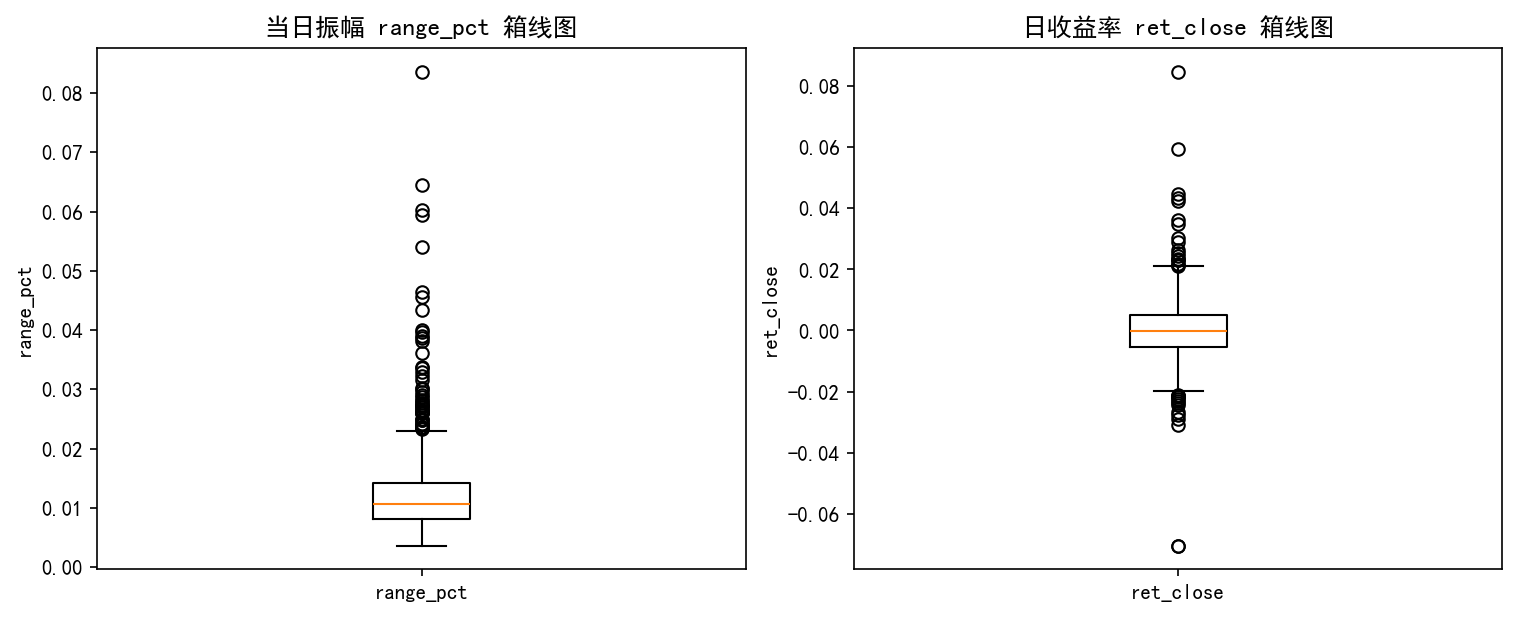
\includegraphics[width=0.85\textwidth]{fig_离群值检测_箱线图.png}
    \caption{离群值检测箱线图（range\_pct、ret\_close 等）}
    \label{fig:box}
\end{figure}
\textbf{原始数据说明}：\texttt{range\_pct} 为当日振幅 (高$-$低)/收盘，反映单日波动幅度；\texttt{ret\_close} 为日收益率，由相邻两日收盘价计算。原始序列中二者均存在极端取值（如单日大涨大跌、振幅异常放大的交易日）。

\textbf{结果分析}：箱线图中箱体表示四分位距（IQR），须线延伸至 1.5$\times$IQR 内的最值，之外为离群点。\texttt{range\_pct} 的箱体集中在较低水平，但存在若干高位离群点，对应波动异常放大的交易日；\texttt{ret\_close} 上下须外均有离群点，对应极端正负收益日（如单日涨跌超过约 5\%--7\% 的交易日）。这说明原始数据中涨跌幅与振幅存在极端值，可能来自重大事件或流动性冲击；线性回归对离群值较敏感，建模时必要时可对尾部截尾或采用稳健方法，并在残差分析中关注这些点的影响。

\begin{figure}[H]
    \centering
    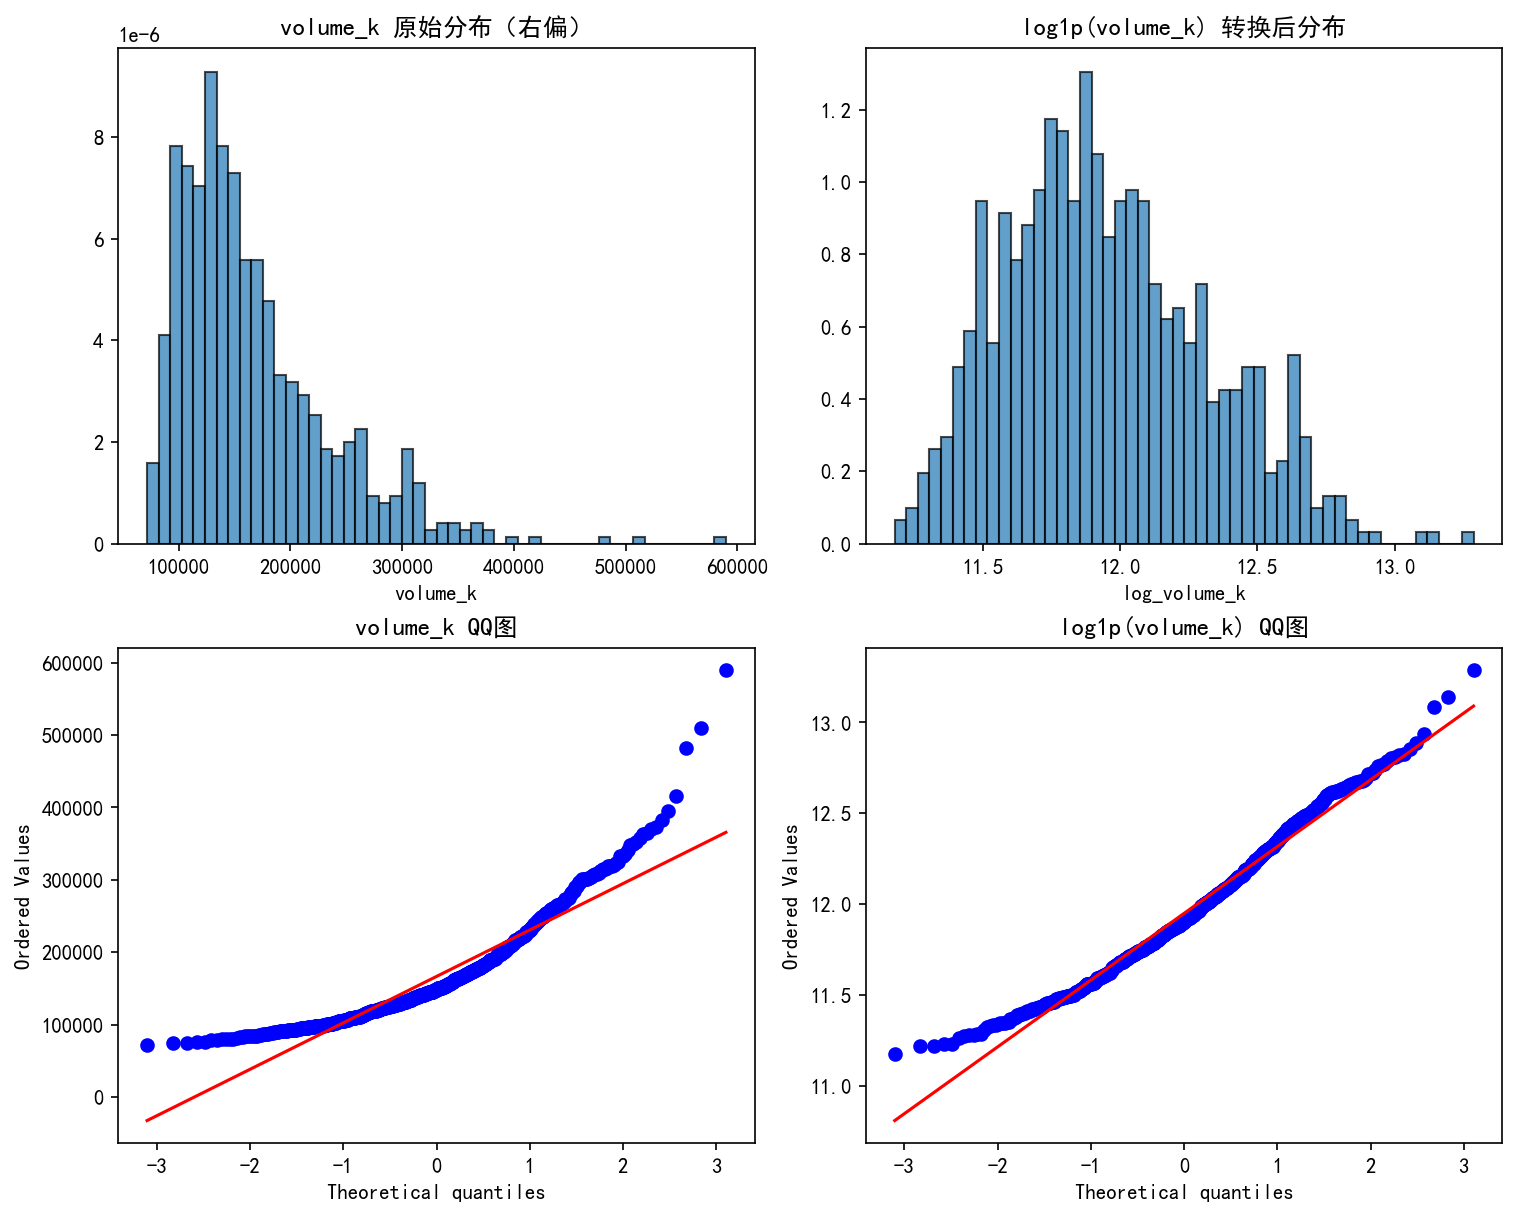
\includegraphics[width=0.85\textwidth]{fig_正态性_对数转换对比.png}
    \caption{正态性：交易量对数转换前后对比（直方图与 QQ 图）}
    \label{fig:norm}
\end{figure}
\textbf{原始数据说明}：原始交易量 \texttt{volume\_k} 以“千”为单位，数值多为正且跨度大，分布往往右偏（少数交易日放量导致长右尾），直接用于回归或假设检验时可能违背正态性假设。

\textbf{结果分析}：左列为 \texttt{volume\_k} 的直方图与 QQ 图。直方图呈明显右偏，右侧拖尾较长；QQ 图中点在中段大致沿参考线，两端尤其是右端明显上翘，偏离“理论正态线”，说明右尾比正态分布更厚。右列为 \texttt{log1p(volume\_k)} 的直方图与 QQ 图。对数转换后直方图更接近钟形，QQ 图上的点整体更贴近对角线，右端偏离减轻。结论：对数转换可改善交易量的正态性、减轻右偏，便于后续将其纳入线性模型或进行基于正态的推断；若不对转换，大成交量交易日可能对回归系数与残差产生较大影响。

\begin{figure}[H]
    \centering
    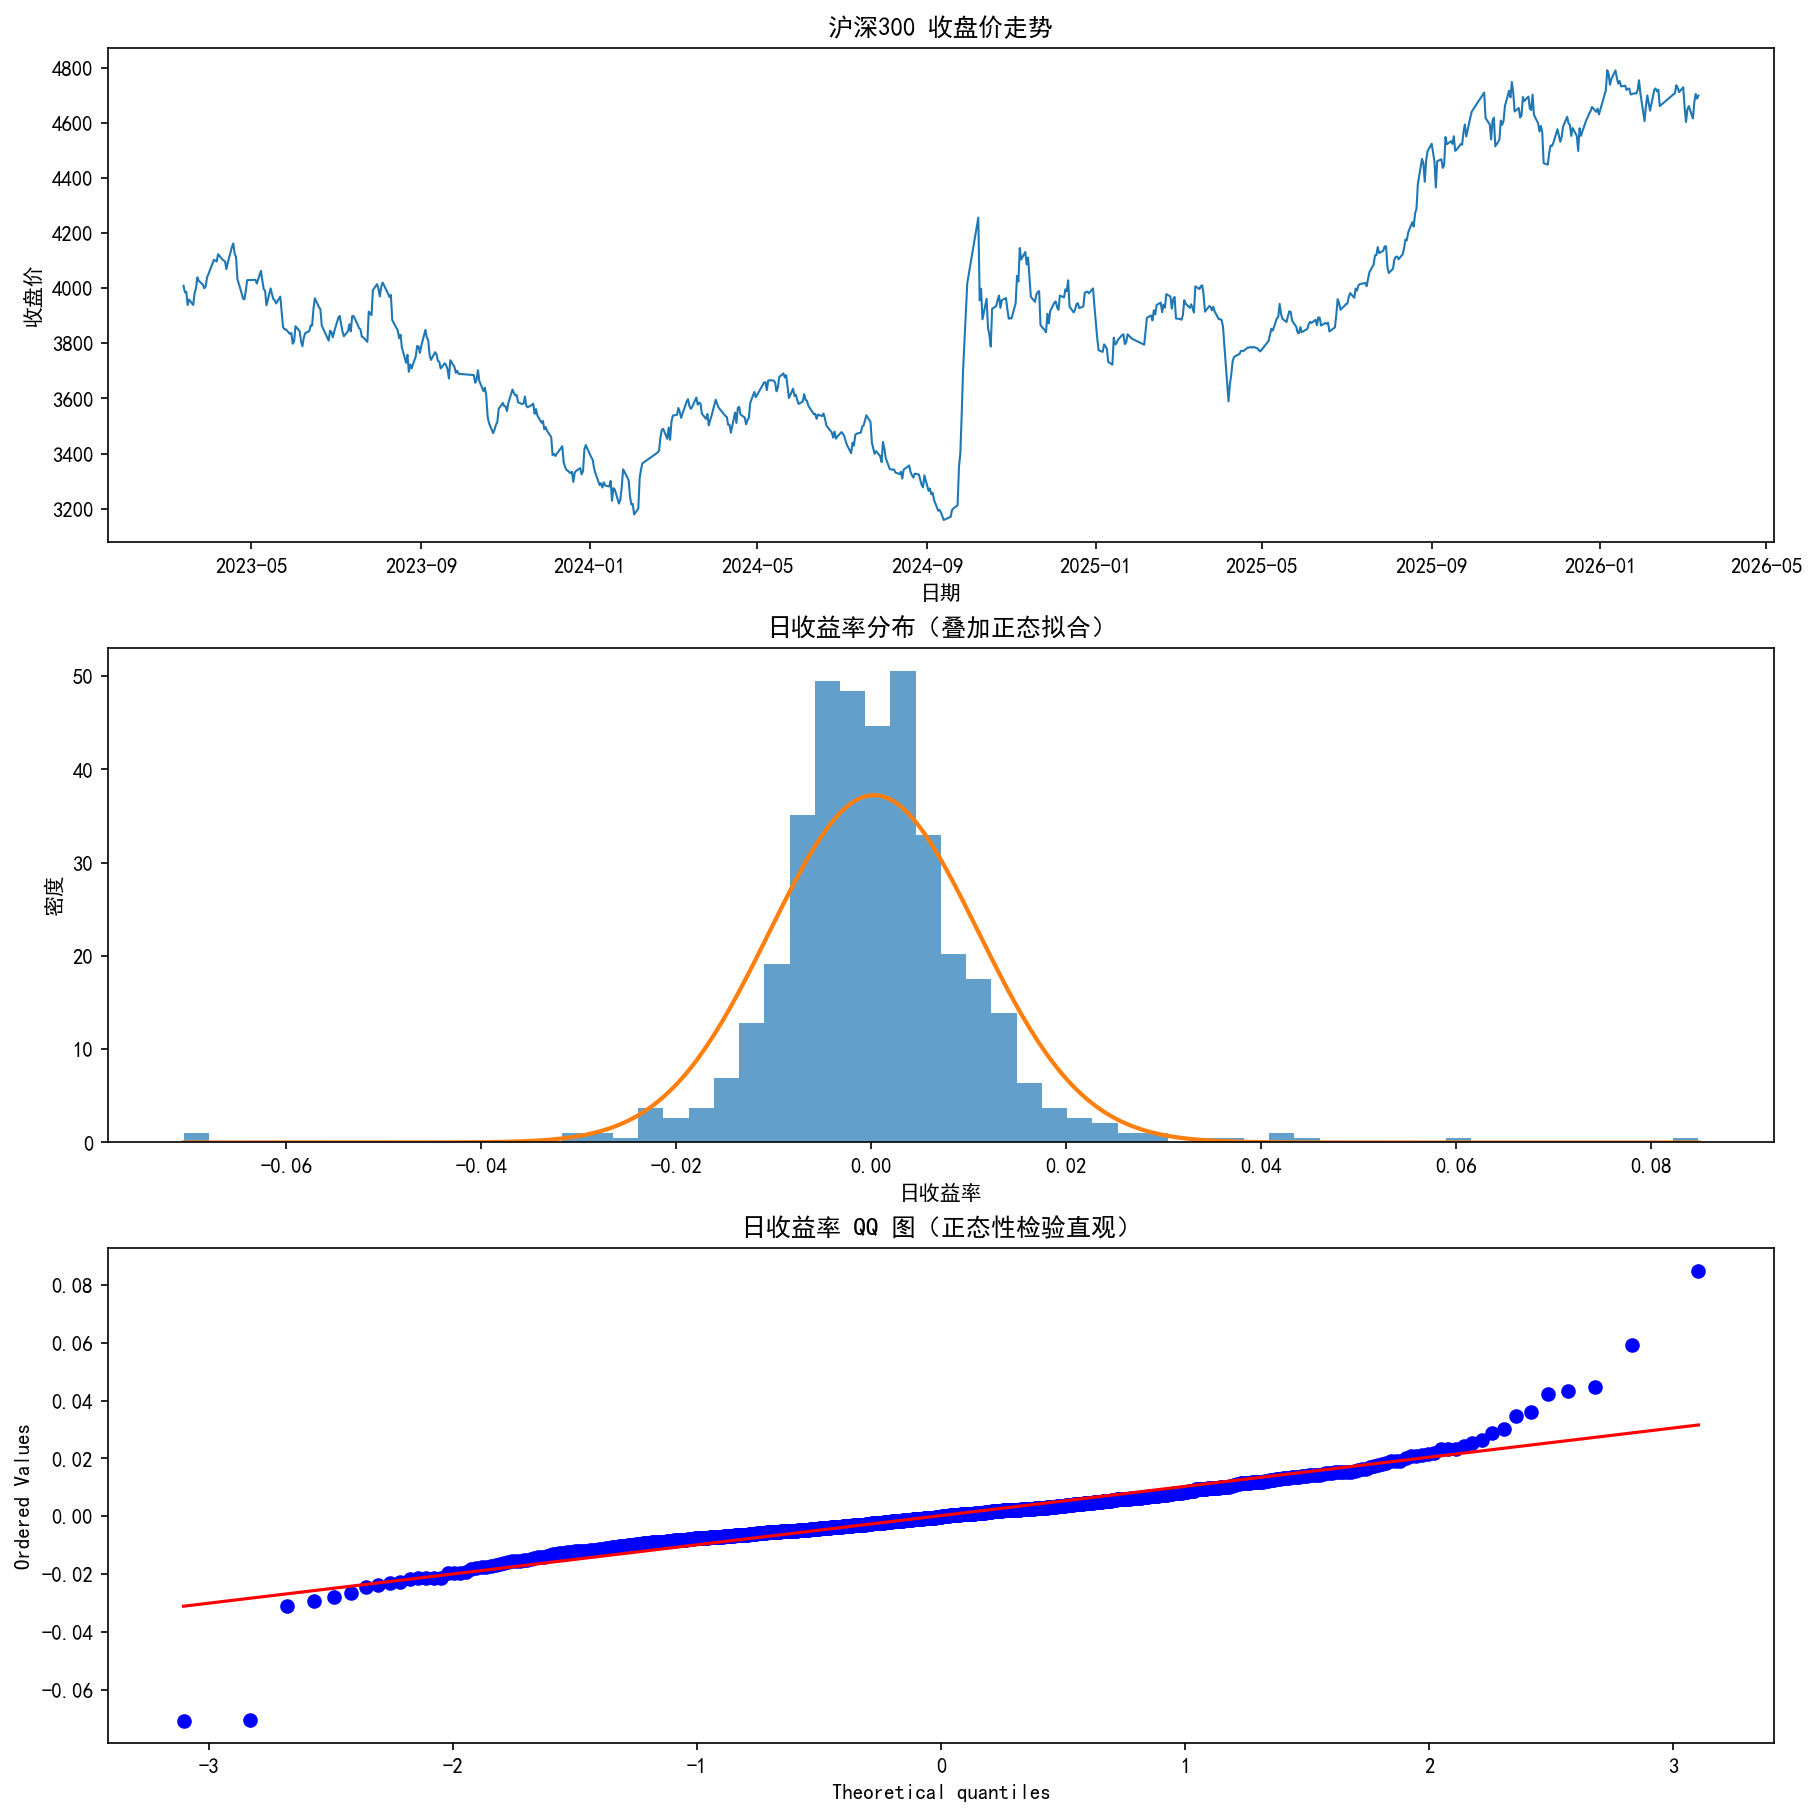
\includegraphics[width=0.85\textwidth]{fig1_收益率分布与QQ图.png}
    \caption{日收益率分布（直方图叠加正态曲线与 QQ 图）}
    \label{fig:ret}
\end{figure}
\textbf{原始数据说明}：日收益率 \texttt{ret\_close} 由原始收盘价序列计算得到，反映指数日度回报。金融中日收益率通常具有“尖峰厚尾”特征：多数交易日收益接近 0，但极端正负收益出现的概率高于正态分布所预测。

\textbf{结果分析}：直方图中心在 0 附近，大部分观测集中在均值两侧，但相比叠加的正态曲线，经验分布峰部更尖、两侧尾部更厚，即“尖峰厚尾”。QQ 图在中间段大致沿对角线，但在左端下弯、右端上翘，对应负收益与正收益的厚尾：极端负收益与极端正收益均多于正态假设下的预期。这与表\ref{tab:desc-ret} 中偏度 0.46、峰度 12.07 的结论一致，说明日收益率明显偏离正态分布。含义：若以 OLS 做回归，残差也可能呈现类似非正态与厚尾，假设检验与置信区间依赖正态假设时需谨慎；可结合残差图与稳健标准误，或考虑对收益率做变换/使用稳健回归方法。

\subsection{相关性分析的结果与分析}

\begin{figure}[H]
    \centering
    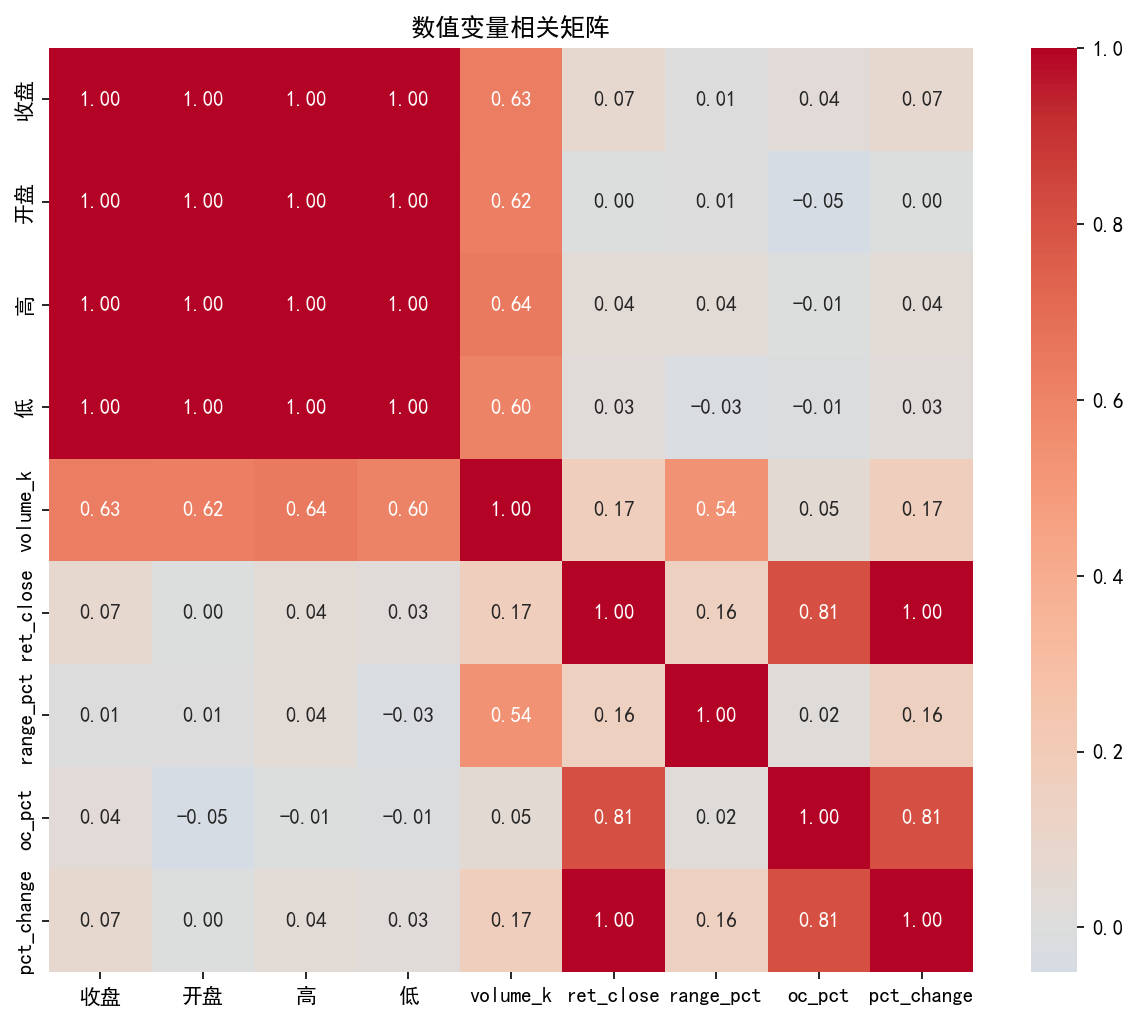
\includegraphics[width=0.8\textwidth]{fig2_相关系数热力图.png}
    \caption{数值型变量相关系数热力图}
    \label{fig:heatmap}
\end{figure}
\textbf{原始数据说明}：参与相关矩阵的变量包括收盘、开盘、高、低、\texttt{volume\_k}、\texttt{ret\_close}、\texttt{range\_pct}、\texttt{oc\_pct} 等数值列，均为原始或衍生后的连续变量，便于计算 Pearson 相关系数。

\textbf{结果分析}：热力图中颜色深浅表示相关系数绝对值大小。可观察到：\texttt{oc\_pct}（开收差）与 \texttt{ret\_close}（日收益率）高度正相关，因二者均反映当日涨跌方向与幅度；\texttt{range\_pct}（振幅）与当日绝对收益率（或与 \texttt{ret\_close} 的某种度量）往往呈正相关，即波动大的交易日其绝对收益的绝对值也倾向于较大；\texttt{volume\_k}（交易量）与其他变量的线性相关相对较弱。这些关系为回归中纳入 \texttt{range\_pct}、\texttt{oc\_pct} 等特征提供了依据；同时 \texttt{oc\_pct} 与 \texttt{ret\_close} 高度相关可能带来多重共线性，回归系数解释时需注意，可结合 VIF 或变量选择进一步分析。

\begin{figure}[H]
    \centering
    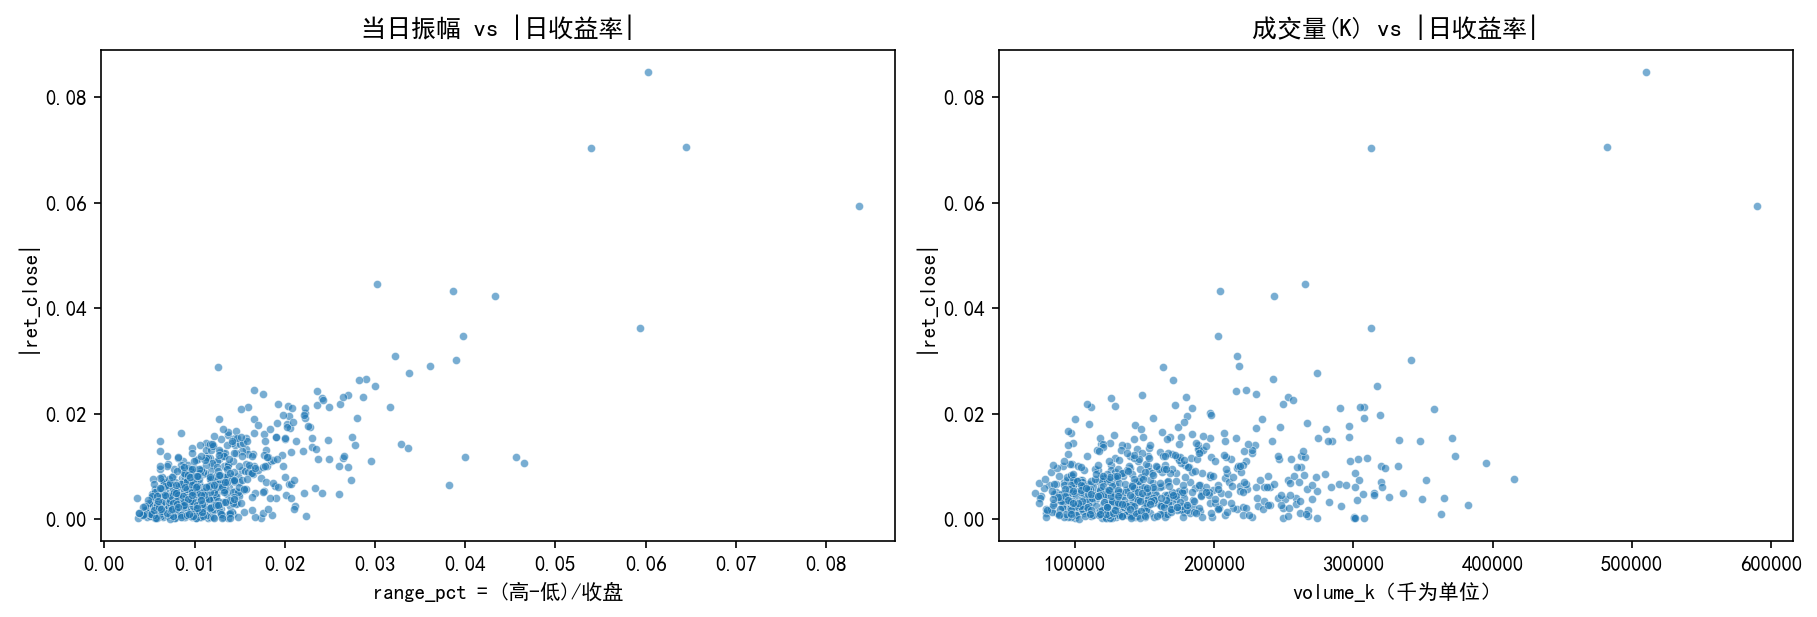
\includegraphics[width=0.8\textwidth]{fig3_振幅与成交量散点图.png}
    \caption{振幅与成交量散点图}
    \label{fig:scatter}
\end{figure}
\textbf{原始数据说明}：横轴为当日振幅 \texttt{range\_pct}，纵轴为交易量 \texttt{volume\_k}（或绝对收益率等）；每个点对应一个交易日，可观察“波动幅度”与“成交活跃度”或“绝对收益”之间的散点形态。

\textbf{结果分析}：若点云呈从左下到右上的带状趋势，说明振幅较大时成交量或绝对收益往往较大，符合“波动放大时交投更活跃”的直觉；若整体趋势不明显或呈非线性，则线性相关系数较弱。本实验散点图若关系较弱，与多元回归中 \texttt{volume\_k} 系数接近 0 的结果一致，即线性意义上成交量对下一日收益率的边际解释力有限。散点图还可帮助识别远离点云的离群日，便于在建模或结果解读时单独关注。

\subsection{简单线性回归分析的结果与分析}
多元线性回归以当日 \texttt{ret\_close}、\texttt{range\_pct}、\texttt{oc\_pct}、\texttt{volume\_k} 为自变量，下一日收益率为因变量，回归系数与模型评估见表\ref{tab:coef} 与表\ref{tab:metrics}。回归方程为：
\[
y = -0.001633 - 0.0970 \times \texttt{ret\_close} + 0.1063 \times \texttt{range\_pct} + 0.2380 \times \texttt{oc\_pct} + 0 \times \texttt{volume\_k}
\]
测试集 $R^2$ 为负，说明模型在样本外解释力很弱，甚至逊于用均值预测；\texttt{volume\_k} 系数接近 0，与相关性及散点图中成交量与收益线性关系较弱的结论一致。

\begin{table}[H]
\centering
\caption{多元线性回归系数与截距}
\label{tab:coef}
\begin{tabular}{lc}
\toprule
变量 & 系数 \\
\midrule
截距 (intercept) & $-$0.001633 \\
ret\_close        & $-$0.0970 \\
range\_pct        & 0.1063 \\
oc\_pct           & 0.2380 \\
volume\_k         & $\approx$0 \\
\bottomrule
\end{tabular}
\end{table}

\begin{table}[H]
\centering
\caption{多元线性回归模型评估（Train / Test）}
\label{tab:metrics}
\begin{tabular}{lcc}
\toprule
指标 & 训练集 & 测试集 \\
\midrule
MSE  & 0.000118 & 0.000092 \\
MAE  & 0.00725  & 0.00758 \\
$R^2$ & 0.0259   & $-$0.0586 \\
\bottomrule
\end{tabular}
\end{table}

\begin{figure}[H]
    \centering
    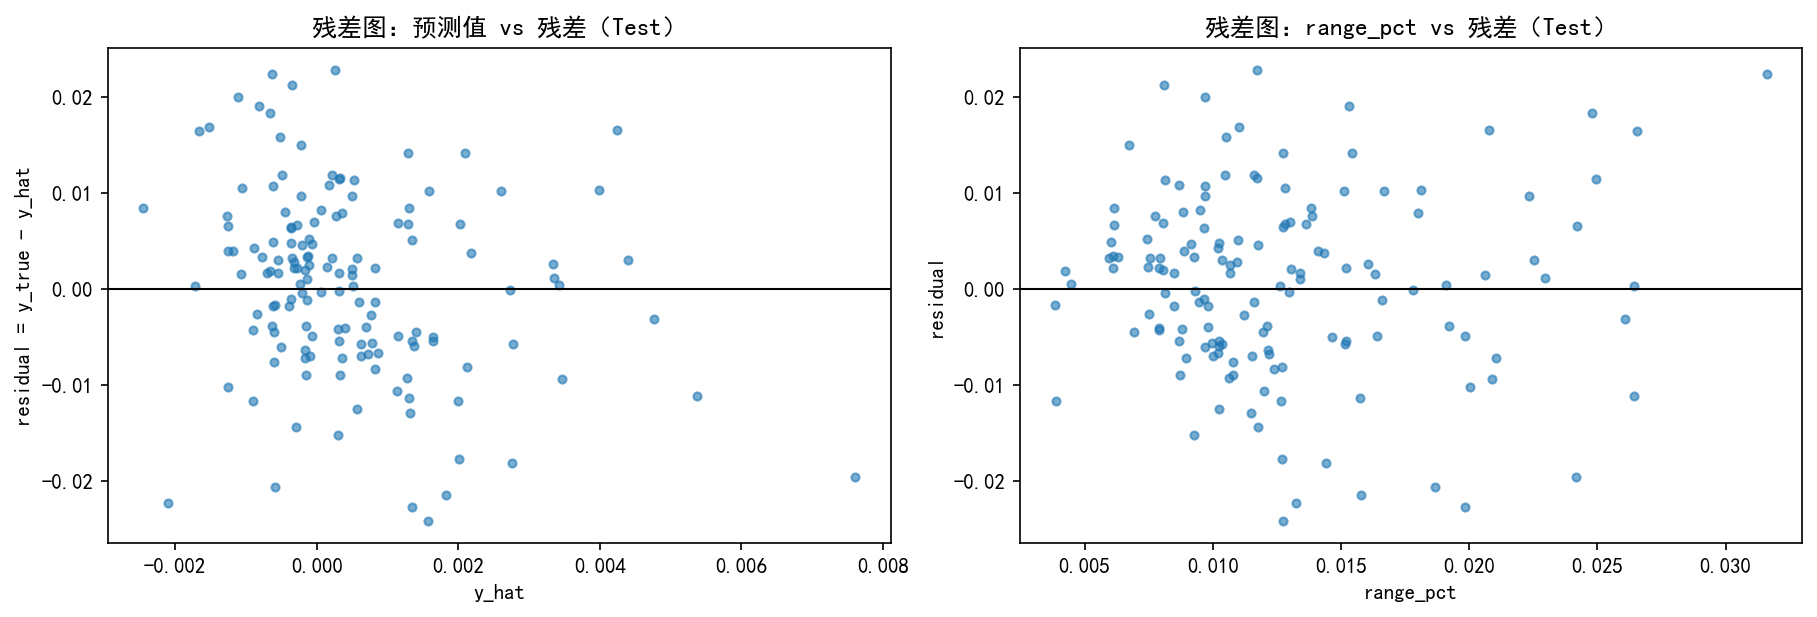
\includegraphics[width=0.85\textwidth]{fig4_残差图.png}
    \caption{多元线性回归残差图}
    \label{fig:resid}
\end{figure}
\textbf{原始数据说明}：残差为测试集上的“真实下一日收益率 $-$ 模型预测值”；横轴可为预测值 \texttt{y\_hat} 或自变量 \texttt{range\_pct}，纵轴为残差。若模型设定与同方差假设成立，残差应围绕 0 随机波动且波动幅度不随横轴系统性变化。

\textbf{结果分析}：左图（预测值 vs 残差）用于检查残差是否随预测值增大而出现“喇叭口”或“漏斗形”，即异方差。右图（\texttt{range\_pct} vs 残差）用于检查残差方差是否随振幅增大而增大。若两图中残差在 0 线两侧大致均匀、带状宽度稳定，则同方差假设大致成立；若在高预测值或高 \texttt{range\_pct} 一侧残差绝对值明显变大，则存在异方差，OLS 标准误可能低估，可考虑稳健标准误或加权最小二乘。此外，日收益率本身具有厚尾特征，残差也可能出现少量远离 0 的点，需结合 Breusch-Pagan 检验综合判断。

\subsection{同方差与异方差的结果与分析}
经典线性回归假设之一为同方差（残差方差恒定）。若残差图呈“喇叭口”或“漏斗形”，即残差绝对值随预测值或自变量增大而增大，则存在异方差。Breusch-Pagan 检验以残差平方对自变量做辅助回归，LM 或 F 的 p-value 若小于 0.05，则拒绝同方差假设。本实验对 Test 集残差做 Breusch-Pagan 检验：若 p < 0.05，则存在异方差，OLS 标准误不可靠，可考虑稳健标准误（如 White、HC）或加权最小二乘（WLS）；若 p $\geq$ 0.05，则未拒绝同方差假设，残差方差相对稳定。结合残差图与检验结果综合判断。

\begin{figure}[H]
    \centering
    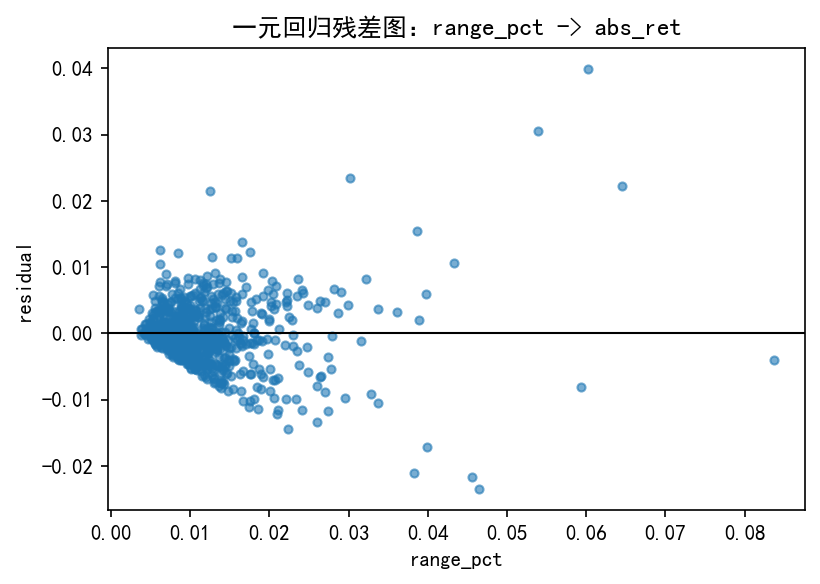
\includegraphics[width=0.85\textwidth]{fig5_一元回归残差图.png}
    \caption{一元线性回归残差图（range\_pct $\to$ abs\_ret）}
    \label{fig:resid1}
\end{figure}
\textbf{原始数据说明}：一元回归以当日振幅 \texttt{range\_pct} 为自变量、当日绝对收益率 \texttt{abs\_ret}（$|$\texttt{ret\_close}$|$）为因变量，用于演示手工计算 $\beta_0$、$\beta_1$ 及残差图解读。二者在定义上存在内在联系：振幅大时当日涨跌幅的绝对值往往也较大，故线性相关较强。

\textbf{结果分析}：手工计算得 $R^2 \approx 0.58$，MSE $\approx 2.59\times10^{-5}$。$R^2$ 较高主要因为 \texttt{range\_pct} 与 \texttt{abs\_ret} 存在内生相关，并非单纯的预测关系，预测意义有限。残差图横轴为 \texttt{range\_pct}，纵轴为残差。若残差随 \texttt{range\_pct} 增大而上下分散程度加大（喇叭口），则存在异方差；若在 0 线两侧大致均匀、带宽稳定，则同方差假设相对可接受。可与多元回归残差图对比：多元回归预测的是“下一日收益率”，一元回归解释的是“当日绝对收益”，二者残差结构可能不同，便于理解不同设定下同方差假设是否成立。

% ========== 六、实验总结 ==========
\section{实验总结}
\begin{enumerate}[leftmargin=*]
    \item \textbf{数据清洗}：完成日期、交易量、涨跌幅的类型转换与衍生特征（\texttt{ret\_close}、\texttt{range\_pct}、\texttt{oc\_pct}）构建；缺失仅首日两列，已在建模时 \texttt{dropna} 处理。
    \item \textbf{缺失与正态性}：缺失数据统计表明确各列缺失情况；正态性检验（Shapiro-Wilk、D'Agostino K²）表明日收益率拒绝正态性，交易量经 \texttt{log1p} 转换后更接近正态。
    \item \textbf{描述性统计与分布}：收盘价分布较对称；日收益率尖峰厚尾、偏度约 0.46、峰度约 12.07。
    \item \textbf{可视化与离群值}：箱线图显示 \texttt{ret\_close}、\texttt{range\_pct} 存在离群值；对数转换与收益率 QQ 图验证了正态性讨论；热力图与散点图揭示了变量间关系，为回归变量选择提供依据。
    \item \textbf{回归与评估}：多元线性回归得到回归方程及 Train/Test 的 MSE、MAE、$R^2$；时间序列前 80\%/后 20\% 划分；测试集 $R^2$ 为负，说明简单线性模型对下一日收益的样本外预测能力不足；一元回归 $R^2$ 较高但与内生性有关，预测意义有限。
    \item \textbf{同方差与异方差}：通过残差图可初步诊断同方差；Breusch-Pagan 检验可正式检验异方差；若存在异方差或厚尾，可考虑稳健标准误、加权最小二乘或非线性/稳健模型。
    \item \textbf{局限性}：\texttt{range\_pct} 与 \texttt{abs\_ret} 存在内生相关；更规范做法可尝试前日特征预测当日收益或 CAPM 等模型；可扩展方向包括技术指标、滚动窗口、非线性模型（如随机森林/GBDT）及残差结构对比。
\end{enumerate}

\end{document}
